\documentclass{assignment}
\begin{document}

\lstset{language=Matlab,%
    %basicstyle=\color{red},
    breaklines=true,%
    morekeywords={matlab2tikz},
    keywordstyle=\color{blue},%
    morekeywords=[2]{1}, keywordstyle=[2]{\color{black}},
    identifierstyle=\color{black},%
    stringstyle=\color{mylilas},
    commentstyle=\color{mygreen},%
    showstringspaces=false,%without this there will be a symbol in the places where there is a space
    numbers=left,%
    numberstyle={\tiny \color{black}},% size of the numbers
    numbersep=9pt, % this defines how far the numbers are from the text
    emph=[1]{for,end,break},emphstyle=[1]\color{red}, %some words to emphasise
    %emph=[2]{word1,word2}, emphstyle=[2]{style},    
}

\assignmentTitle{Emil Sønderskov Hansen}{20196042}{assets/logo.png}{Sound Processing}{Mini-Project: Efficient HRTF filter for 3D sound}

\section*{Intro}

\begin{figure}[h]
    \centering
    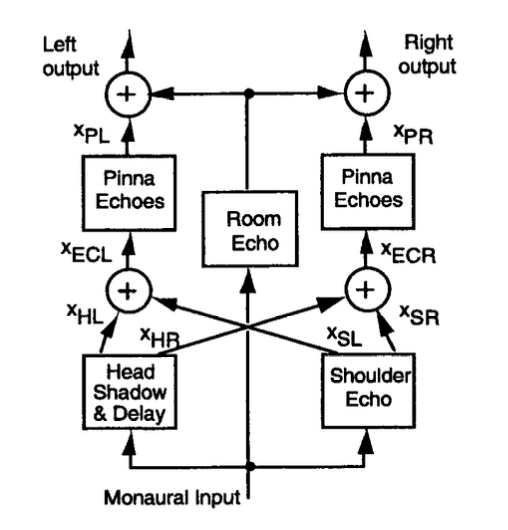
\includegraphics[scale = 0.3]{assets/HRTF.png}
    \caption{All of the components of the HRTF model}
    \label{fig:theModel}
\end{figure}

In the HRTF model proposed by Brown and Duda, various modules simulate different aspects of sound. The model's purpose is not to replicate physical processes but to create a simple system that can effectively convey impressions of spatial dimensions. The model takes a monaural input and processes it through a head model, followed by a pinna model, to produce azimuth and elevation effects. Additionally, the output from a room model is incorporated to generate range effects. In this project, a MatLab implementation of the head, pinna, and room models is presented and combined to create a complete HRTF model, as seen in figure \ref{fig:theModel}. The paper found the shoulder model (from figure \ref{fig:theModel}) to provide weak localization cues, which was therefore omitted from the paper and this implementation. 

\section*{The Head Model}

\begin{figure}[h]
    \centering
    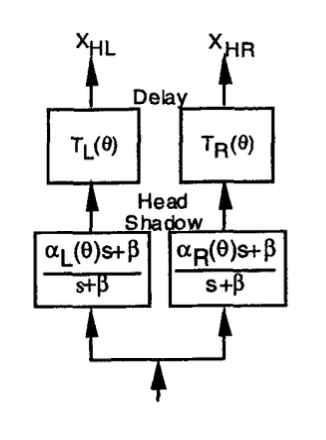
\includegraphics[scale = 0.4]{assets/HeadModel.png}
    \caption{The components of the head model}
    \label{fig:headModel}
\end{figure}

As seen in figure \ref{fig:headModel}, the Head Model splits the signal to left and right. And each signal then goes through a Head Shadow filter (Interaural Level Difference (ILD)) and a delay (ITD). \newline

\paragraph{Head Shadow filter \newline}

The Head Shadow filter is introduced in the paper as an analog one-pole/one-zero transfer function, as follows: 

\[H(s,\theta)=\frac{\alpha(\theta)s + \beta}{s + \beta}, where \beta = \frac{2c}{a}\]

The transfer function has a fixed pole at  $-\beta$ and a zero depending on the azimuth value. The value of $\alpha$ is dependent on whether the input is the left or the right signal; $\alpha$$_{L}(\theta) = 1 - sin(\theta)$ and $\alpha$$_{R}(\theta) = 1 + sin(\theta)$. \newline

The proposed transfer function is analog (i.e., a continuous time transfer function), and a digital version (i.e., discrete-time version) was approximated using a bilinear transform (also called the Tustin method). The bilinear transform states that the digital version can be derived by $s = \frac{2}{T}\frac{z-1}{z+1}$. The following is the approximated discrete-time transfer function.

\[H(z,\theta)=\frac{\alpha(\theta) + T\beta + z^{-1}(-2\alpha(\theta) + T\beta)}{2 + T\beta+z^{-1}(-2 + T\beta)}\]

And from the transfer function, the difference equation can be derived and is used in the Matlab Head Shadow function (see code below). 

\[y(n) = \frac{(2\alpha(\theta) + T\beta)x(n) + (-2\alpha(\theta) + T\beta)x(n-1) - (-2 + T\beta)y(n-1)} {2 + T\beta}\]

This difference equation gave the desired results and contributed to useful localization cues.\newline

It was also attempted to use the build-in Matlab function \textit{c2d(system,T,'tustin')} followed by the function \textit{impulse(system)} instead, to create an impulse response to convolute with the input signal. However, this did not give the desired result for unknown reasons and distorted the system heavily (this code is also attached). \newline


The full derivations can be found in the appendix.

\lstinputlisting{assets/HeadShadow.m}

\paragraph{Delay \newline}

The two delays are calculated based on the radius on the radius of the head (a), the azimuth ($\theta$), and the speed of the sound (c). The article proposed the following calculations for delay for left and right and is implemented in the code: 

\[T_{L}(\theta) = \frac{a + a\theta\ }{c},  T_{R}(\theta) = \frac{a - asin(\theta) }{c}\]

The delays are calculated and multiplied by the sampling rate of the input to find the number of samples to delay the signal with. The calculated was floored to an integer, providing the ITD cues good enough. Adding fractional delay did not seem to provide any further cues. The Matlab implementation can be seen below.

\lstinputlisting{assets/ITD.m}

\section*{Pinna Echoes}

\begin{figure}[h]
    \centering
    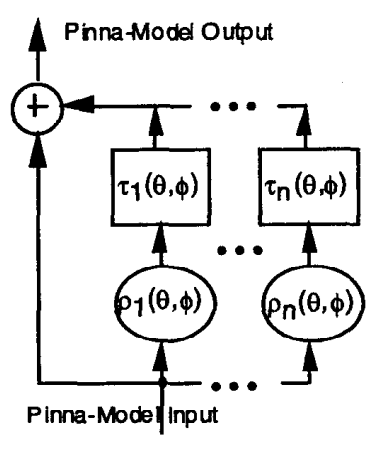
\includegraphics[size = 0.7]{assets/pinnamodel.png}
    \caption{The model to represent the Pinna Echoes of five different events (i.e., time delays)}
    \label{fig:pinnaModel}
\end{figure}

While the Head Model provides cues for azimuth, the Pinna Model (see figure \ref{fig:pinnaModel}) provides elevation cues (as it is dependent on elevation ($\phi$)). The pinna echoes are represented by five events (i.e., time delays) by $\tau_{k}$, which each have an amplitude of $\rho_{k}$. The time delays for the five events are calculated with the following equation: 

\[\tau_{k}(\theta,\phi) = A_{k}cos(\frac{\theta}{2})sin(D_{k}(90^{\circ} - \phi)) + B_{k}\]

\begin{figure}[h]
    \centering
    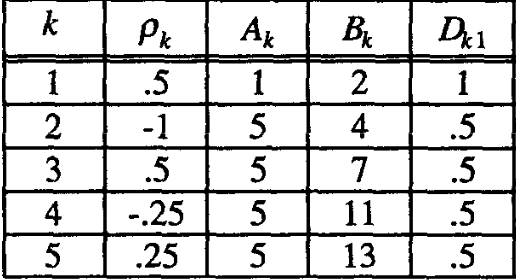
\includegraphics[scale = 0.8]{assets/coeffecient.png}
    \caption{Pinna Echo coefficients proposed by the paper}
    \label{fig:coefficients}
\end{figure}

The article proposes coefficients used for calculating the delays. The coefficients are shown in figure \ref{fig:coefficients}. \newline

A finite impulse response (FIR) was implemented to represent the pinna echoes. Firstly, all delays are calculated, and then an empty FIR with the number of taps of the highest delay is created. The first FIR tap is set to 1 as the input signal passes through (see figure \ref{fig:pinnaModel}). Each event is then placed in the impulse response based on the calculated delays with a value of $\rho_{k}$. In the implementation, it was tried to floor the delay to an integer. However, this did not seem to provide precise cues for elevation. The cues were found to be more accurate when distributing the value of $\rho_{k}$ on two samples based on the fraction of the delay. Lastly, the input is convoluted with the impulse response. The elevation cues from the impulse response were not perceived as completely accurate. However, it must be considered that the article mentions $D_{k}$, to be adapted to the individual listener. The Matlab implementation can be seen below

\lstinputlisting{assets/PinnaEchoFunction.m}

\section*{Room Model}

\begin{figure}[h]
    \centering
    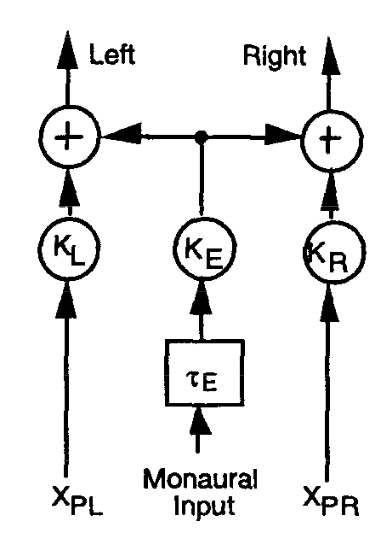
\includegraphics[scale = 0.7]{assets/mono.png}
    \caption{The Room Model}
    \label{fig:roomModel}
\end{figure}

The room model proposed in the paper is simply the original mono signal delayed and gained down (see figure \ref{fig:roomModel}). Firstly the signal is delayed by $\tau_{E}$ proposed to be 15 ms. And afterward gained down by $K_{E}$ to be 15db lower than the channel gains $K_{L}$ and $K_{R}$. \newline

A gain for the channels was implemented, and the gain of the room model was fixed to be 15 dB lower. The code can be seen below. 

\lstinputlisting{assets/RoomModel.m}

\section{The full HRTF code}

All the different functions were gathered in one HRTF function as seen below: 

\lstinputlisting{assets/HRTF.m}

\newpage
\section{Appendix}2r

\subsection{Head Shadow Model: Discrete-time transfer function}
\begin{figure}[h]
    \centering
    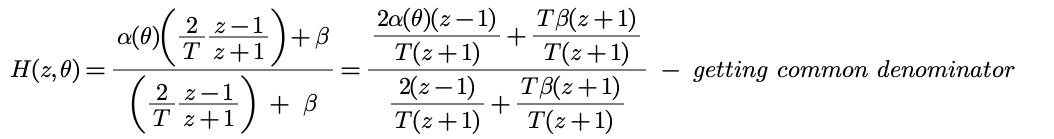
\includegraphics[scale=0.5]{assets/b1.png}
    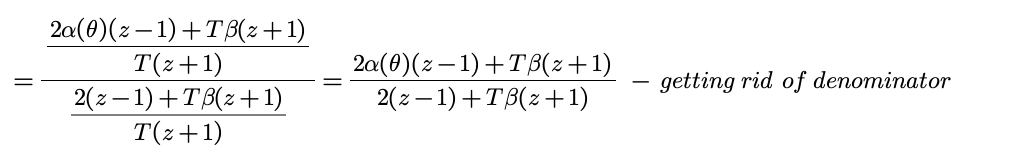
\includegraphics[scale=0.5]{assets/b2.png}
    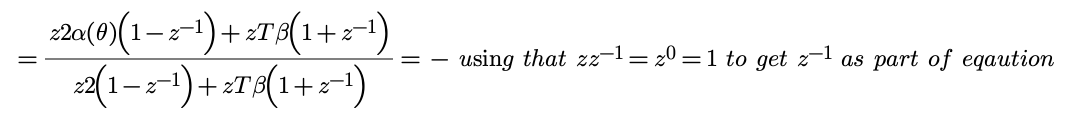
\includegraphics[scale=0.5]{assets/b3.png}
    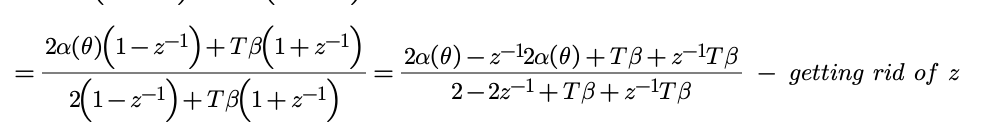
\includegraphics[scale=0.5]{assets/b4.png}
    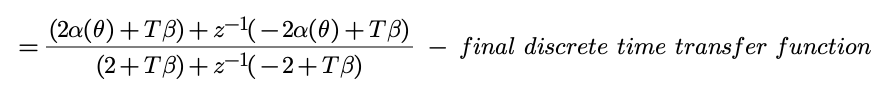
\includegraphics[scale=0.5]{assets/b5.png}
    \caption{Billinear transform to approximate the discrete-time transfer function from the continuous-time transfer function}
    \label{fig:my_label}
\end{figure}

\newpage 
\subsection{Head Shadow Model: Difference equation derivation}
\begin{figure}[h]
    \centering
    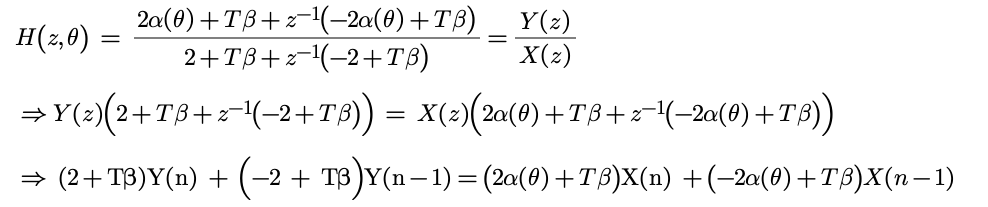
\includegraphics[scale=0.5]{assets/diff1.png}
    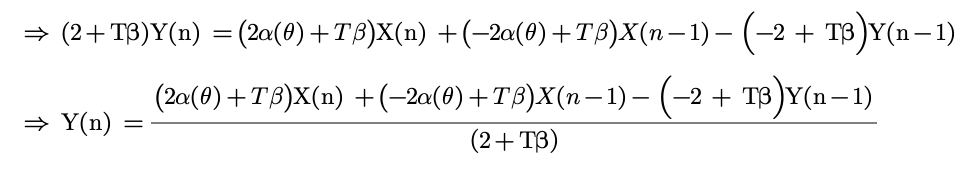
\includegraphics[scale=0.5]{assets/diff2.png}
    \caption{Difference equation derived from the approximated discrete-time transfer function}
    \label{fig:my_label}
\end{figure}

\end{document}
